In the previous section we analyzed the design of the original RSA model, spelled out the relation and distinction between belief, goal and action, and proposed a familiy of alternative models based on different interpretation of these notions. This gives rise to a series of interesting empirical questions regarding the underlying assumptions of the models. In order to gain insight into these questions by comparing the predictive power of different models, we conducted the following experiment to collect empirical data, which we will use to test the predictions of different models in the next section.

There are four major designs in our own experiment that differ from the original experiment in \cite{Frank}. First of all, the original experiment used the betting paradigm, i.e. participants were asked to bet over a range of options and they were instructed that the amount of money that is bet on an option should reflect their confidence that the option is correct. Even though the betting paradigm has the merit of providing us with graded reponses from each individual participant, the caveat is that it is unclear whether it measures the belief or the action. This can lead to confusion when we are to fit the model predictions to the empirical data without knowing whether they are directly comparable. In addition, since the betting paradigm is more or less introspective in nature, it tends to be not very accurate. Thus we used forced choice in our experiment instead, which clearly measures the action and does not rely on introspection.
Secondly, since we decided to investigate the influence of the speaker's preference as well as the listener's perceptual salience, we focused on contexts equivalent to Figure \ref{context}, which are most typical in Gricean accounts of scalar implicature, and examined different features separately.
Thirdly, we only included the features of color and shape to ensure the vocabulary to be common knowledge, excluding the feature of texture. Finally, we did not use dotted line surrounding an object as the way to indicate the target to the speaker, as it could emphasize the feature of shape and thus add confound in the experiment. Instead we used a small arrow pointing to the target. Despite these differences, the remaining aspects in our experiment were almost identical to those of the original one, e.g. the phrasing of the instructions. We also counterbalanced the positions,  colors, and word orders in each condition.

The results of the three parts of our experiment are as follows.

\subsection{Prior Estimation}
We recruited 240 US participants via Amazon Mechanical Turk and presented them with a context of three objects (Figure \ref{exp_context} as an example).  

\begin{figure}[htb] 
  \centering
  \subfigure[A sample context]{\label{exp_context}
  
\begin{tikzpicture}
     \path (-1.4, 0) node [shape=rectangle, draw=green!65 ,fill= green!65 ,minimum size=28]{}
           ( 0, 0) node  [shape=circle, draw=green!65, fill= green!65,minimum size=30] {}
           ( 1.4, 0) node [shape=circle, draw=blue!65, fill=blue!65  ,minimum size=30] {}
     ;
           
  \end{tikzpicture}
  
  }  
  \hspace{5mm}
  \subfigure[Choice distribution]{\label{table:prior}
  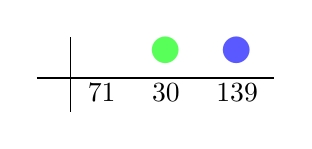
\begin{tikzpicture}
     \path (0,0) node[] 
     {\begin{tabular}{c|ccc}
    \quad &\textcolor{green!65}{\Large{$\blacksquare$}}\quad & \textcolor{green!65}{\Huge{$\bullet$}}\quad & \textcolor{blue!65}{\Huge{$\bullet$}} \\ 
     \hline
     & $71$        &   $30$       & $139$        
     \end{tabular}
     } ;
  \end{tikzpicture}
  }
  \caption{Prior Estimation}
\end{figure}

Participants were instructed to imagine that someone was talking to them and referring to one of the objects, using a foreign language they do not understand. Then they were asked to choose the object they thought that person was talking about. The numbers of participants choosing each object are shown in Figure \ref{table:prior}. We will use this empirical distribution to estimate the perceptual salience prior of each object.

\subsection{Speaker Conditions}

We recruited 432 US participants via Amazon Mechanical Turk in the speaker conditions, 144 in each condition. The participants were presented with a context similar to Figure \ref{exp_context}, with a small arrow indicating the target. The participants were then asked to imagine they were talking to someone else and to choose from the two literally true words to refer to the target object.

\begin{table}[htb]   
  \caption{Speaker Conditions}
  \centering
  \begin{tabular}{c|cccc}
   Target  & ``Green'' & ``Square'' & ``Blue'' & ``Circle'' \\ 
     \hline
\textcolor{green!65}{\Large{$\blacksquare$}}    & $9$        &   $135$   & -- & -- \\
\textcolor{blue!65}{\Huge{$\bullet$}}           & --        &   --      & $119$ & $25$\\
\textcolor{green!65}{\Huge{$\bullet$}}          & $63$        &   --    &  --   & $81$             
  \end{tabular}

  \label{table:speaker}
\end{table}

The numbers of participants choosing each message in each condition are shown in Table \ref{table:speaker}. Note that when the target was the object with the unique shape (as in the first row of the table), the feature of shape (``Square'' in the example) should be the optimal utterance because the listener could uniquely identify it. Similarly when the target was the object with the unique color (the second row), the optimal utterance would be the feature of color (``Blue''). When the target was the object with both features shared, both features should be equally ambiguous because of the context's symmetric nature.

From the data in Table \ref{table:speaker}, we can see that the speakers tend to choose the optimal feature more often when the target has the unique shape than when it has the unique color ($\chi^2=8.5, p<.01$). Even though they seem to prefer the feature of shape when the target's both features are shared, the difference is not statistically significant from uniform random choice ($\chi^2=2.25, p=.13$).


\subsection{Listener Conditions}

We recruited 360 US participants via Amazon Mechanical Turk in the speaker conditions, 180 in each condition. The participants were presented with a context similar to Figure \ref{exp_context}, together with a word denoting either of the shared features (color or shape). The participants were asked to imagine someone else was talking to them and he used the word to refer to one of the objects. Then they were asked to choose the object they thought that person was talking about.

\begin{table}[htb] 
  \caption{Listener Conditions}
  \centering
\begin{tabular}{c|ccc}
   & \quad \textcolor{green!65}{\Large{$\blacksquare$}}&  \textcolor{green!65}{\Huge{$\bullet$}}& \textcolor{blue!65}{\Huge{$\bullet$}} \\ 
     \hline
 ``Green''   \quad  & \quad  $65$      \quad    &   $115$    \quad     & $0$      \\
 ``Circle''   &  \quad $1$        &    $62$        & $117$
  \end{tabular}

  \label{table:listener}
\end{table}

The numbers of participants choosing each object upon hearing each word are shown in Table \ref{table:listener}. Note that in either case, the object with both features shared (the green circle) is what the Gricean pragmatic account predicts to be the target.

The result in Table \ref{table:listener} shows that when the message is ``Green'', listeners prefer the green circle which is predicted by the Gricean pragmatics, while they tend to stick to the blue circle which is more perceptually salient when the message is ``Circle''\footnote{Admittedly it is strange that one participant chose the square when the message was ``Circle''. However, since he passed the attention check we just include his data as it is.}. The behavioral patterns in both conditions are significantly different from uniform random choice, and they significantly differ from each other in respect of whether they conform to the predictions by Gricean pragmatic theory.

